\documentclass[11pt, a4paper, twocolumn]{article}

% Fonts and math (Elsevier-like Times style)
\usepackage{graphicx} % Required for inserting images
\usepackage{array} % For extra column formatting
\usepackage{amsmath, amssymb, cancel, siunitx, mathtools, physics2, upgreek} % for equation environment
\usepackage{float,geometry,subcaption, longtable}
\geometry{margin=2cm}
\usepackage[skip=10pt]{parskip}
\usepackage{setspace}
\usepackage{hyperref, cleveref}
\usepackage{cite, bookmark}
\usepackage{url}
\usepackage[table,xcdraw]{xcolor}
\usepackage[export]{adjustbox}
\usepackage{listings,pdfpages}
\usepackage{dblfloatfix}
\usepackage[en-GB]{datetime2}

% --- Abstract styling (elsarticle look)
\usepackage{abstract}
\renewcommand{\abstractnamefont}{\normalfont\bfseries}
\renewcommand{\abstracttextfont}{\normalfont}
\renewenvironment{abstract}{%
  \par\noindent\rule{\linewidth}{0.4pt}\par
  \begin{center}\bfseries Abstract\end{center}%
}{%
  \par\rule{\linewidth}{0.4pt}\par
}

% --- Section styling (similar to elsarticle
\usepackage{titlesec}
\titleformat{\section}{\normalfont\large\bfseries}{\thesection.}{0.5em}{}
\titleformat{\subsection}{\normalfont\normalsize\bfseries}{\thesubsection.}{0.5em}{}

% Table of contents styling
\usepackage{tocloft}
\cftsetindents{section}{0em}{2em}
\cftsetindents{subsection}{1em}{2em}
\renewcommand\cfttoctitlefont{\hfill\Large\bfseries}
\renewcommand\cftaftertoctitle{\hfill\mbox{}}
\renewcommand\cftfigfont{\footnotesize}
\renewcommand\cftfigpagefont{\footnotesize}
\renewcommand\cftloftitlefont{\large}

\graphicspath{ {./images/} }

\definecolor{blurple}{HTML}{5865F2}
\definecolor{backcolour}{HTML}{272823}

\hypersetup{
    colorlinks=true,
    linkcolor=black,
    urlcolor=black,
    citecolor=blurple,
}

\urlstyle{same}

\DeclareMathOperator{\sinc}{sinc}

\renewcommand{\arraystretch}{1.4}

% Python code export
\lstset{
    language=Python,
    basicstyle=\ttfamily\scriptsize,
    keywordstyle=\color{magenta},       
    commentstyle=\color{gray},        
    stringstyle=\color{teal},  
    showstringspaces=false,
    frame=single,
    breaklines=true,
    numbers=left,
    numberstyle=\tiny\color{gray},
    xleftmargin=4ex
}

\setcounter{secnumdepth}{5}
\setcounter{tocdepth}{5}

\hbadness=99999

%%%%%%%%%%%%%%%%%%%%%%%%%%%%%%%%%%%

\title{%


\includegraphics[width=0.2\linewidth]{ucd_brandmark_black.jpg} \vspace{0.5cm}\\

{\Large\bfseries UCD School of Physics}\vspace{1.5cm}\\

{\large PHYC40600 Physics Astronomy and Space Lab II}\\
{\bfseries Newton's Cooling}

}
\author{Joana C.C. Adao \\ \small Student No.: 23311051}
\date{\today}

\begin{document}

% Title page - single column
\onecolumn
\maketitle

% Abstract - single column
\pagenumbering{roman}
\setcounter{page}{1}
\begin{abstract}

This experiment investigated an aluminium rod heated at one end with lateral Newtonian losses acting on it, to test the temperature profile approaching a steady-state and Prigogine's nonequilibrium minimum entropy theorem. Sixteen calibrated thermocouples recorded the temperature distribution over a 75 minute measurement window with different initial conditions (uniform vs. non-uniform, locally pre-heated). The steady-state profile in both runs were well described by an exponential decay, yielding a decay constant of $\beta = 2.8216\;\pm 0.0264\; m^{-1}$ (uniform) and $2.8042\;\pm 0.0261\; m^{-1}$ (non-uniform), consistent within uncertainty despite the differing initial conditions. The entropy production rate $d_iS/dt$ remained non-negative throughout the runs and decreased monotonically to a non-zero steady-state minimum ($0.2086\;\pm 0.0091$ and $0.2186\;\pm 0.009$), confirming both the second law and Prigogine's theorem, though $-d_eS/dt$ crossed and slightly exceeded $d_iS/dt$ by the end of the run rather than completely converging onto it exactly.

\end{abstract}

\newpage

% Table of Contents - single column
\tableofcontents

\newpage

%%%%%%%%%%%%%%%%%%%%%%%%%%%%%%%%%%%

% Start main content in two columns
\twocolumn
\pagenumbering{arabic}
\setcounter{page}{1}

\section{Introduction} \label{sec:1}

Classic thermodynamics often assumes and describes systems in equilibrium, where temperature and pressure variables are typically uniform and time-independent. However, real systems are almost never in true equilibrium. Instead, they are driven by continuous fluxes in energy or matter until they settle into a nonequilibrium steady state. The way systems approach and behave in these states will be explored. \cite{lurie1980concepts,rafols1992heat}

\subsection{Heat Conduction \& Lateral Newtonian Losses} \label{sec:1.1}

The conservation of heat in a solid, following Fourier's law of heat conduction $\mathbf{J}_q=-\lambda\nabla T$, gives the general differential equation describing the heat distribution in the rod \cite{rafols1992heat,diaz1990heat}:

\vspace{-3ex}
\begin{equation} \label{eq:1}
  \rho c \; \frac{dT}{dt} = \nabla \cdot (\lambda \nabla T)
\end{equation}

with $\rho$ as the density, $c$ as the specific heat, and $\lambda$ as the thermal conductivity of the rod. For a rod losing heat through its lateral surface to an external bath of temperature $T_R$, Newton's law of cooling is implemented as the boundary condition \cite{rafols1992heat,diaz1990heat}:

\vspace{-3ex}
\begin{equation} \label{eq:2}
  \lambda \; \mathbf{\hat{\rho_0}} \cdot (\nabla T) + H(T-T_R) = 0
\end{equation}

This states that the normal heat flow through the surface of the rod is proportional to the difference in temperature with respect to the external bath. Here, $H$ is the surface conduction, and $\hat{\rho_0}$ is the outward radial (normal) unit vector. \cite{diaz1990heat,rafols1992heat}

When the rod's thermal conductivity is high relative to its radius, the radial temperature gradients remain small relative to its axial variation. Averaging across the rod's cross-section then folds this boundary condition into an effective source term within a purely one-dimensional equation \cite{diaz1990heat,rafols1992heat}:

\vspace{-3ex}
\begin{equation} \label{eq:3}
  \rho c \; \frac{\partial T(z,t)}{\partial t} = \lambda \frac{\partial^2 T(z,t)}{\partial z^2} - \frac{2H}{r} [T(z,t)-T_R]
\end{equation}

with $r$ as the rod's radius. This equation interpolates between the two limits of the boundary condition discussed for the rod: for $H \to 0$ representing a perfectly insulating surface, and $H\to \infty$ representing a perfectly conductive surface. \cite{rafols1992heat}

Under a fixed boundary temperature difference, the rod cannot relax to equilibrium. Instead, it approaches a time-independent, nonequilibrium steady state given as $T_{SS}(z)$, which is found by setting $\partial T/\partial t = 0$ \cite{rafols1992heat}:

\vspace{-3ex}
\begin{equation}\label{eq:4}
  [T_{SS}(z, \infty)-T_R] = [T_L-T_R]\; e^{-\beta z}
\end{equation}

with $T_L$ as the extrapolated boundary temperature at $z=0$, and the coefficient $\beta$ given by $\beta=\sqrt{2H/\lambda r}$. As $\beta$ depends only on the thermal and geometric properties of the rod and its surroundings ($H$, $\lambda$, $r$), it is treated as a constant that can be purely experimentally determined from the steady-state temperature distribution. \cite{diaz1990heat,rafols1992heat}

\subsection{Nonequilibrium Thermodynamics} \label{sec:1.2}

In thermodynamics, entropy is defined only for states in thermodynamic equilibrium. Therefore, to extend this to a nonequilibrium system, the local equilibrium hypothesis is considered: the system is subdivided into volume elements that are each large enough to have well-defined temperatures and pressures, yet small enough that these values do not vary appreciably within the element. Gibbs' relation is assumed to hold for each element \cite{rafols1992heat}:

\vspace{-3ex}
\begin{equation}\label{eq:5}
  ds=\frac{1}{T}du
\end{equation}

with $s$ and $u$ as the entropy and internal energy, respectively. When combined with the local energy balance it yields the local entropy balance equation \cite{lurie1980concepts,rafols1992heat}:

\vspace{-3ex}
\begin{equation} \label{eq:6}
  \rho \frac{ds}{dt} + \nabla \mathbf{J_s} = \sigma
\end{equation}

with $\mathbf{J_s} = \mathbf{J_q}/T$ as the entropy flux density, and $\sigma =\mathbf{J_q} \cdot \nabla (1/T)$ as the local entropy production. The second law of thermodynamcis requires $\sigma \ge 0$ at every point. \cite{lurie1980concepts,rafols1992heat}

Integrating over the whole rod separates the entropy change into two physically distinct contributions \cite{lurie1980concepts,rafols1992heat}:

\vspace{-3ex}
\begin{equation} \label{eq:7}
  \frac{dS}{dt} = \frac{d_eS}{dt} + \frac{d_iS}{dt}
\end{equation}

with $d_eS/dt$ as the entropy exchanged with the surroundings across the system's boundary, and $d_iS/dt$ as the exchanges inside the system. The second law thus requires that $d_iS/dt \ge 0$ at all times, with equality only possible for reversible processes. \cite{rafols1992heat,prigogine1978time}

\subsection{Minimum Entropy Production} \label{sec:1.3}

Near equilibrium, the thermodynamic heat flux $J$ relates linearly to its conjugate force $X=\nabla (1/T)$ by $J=LX$. When several fluxes and forces are present, the Onsager reciprocal relations $L_{ij}=L_{ij}$ govern the coupling between them. \cite{lurie1980concepts,onsager1931reciprocal} Within this linear regime, Prigogine's theorem of minimum entropy production states that a system relaxing toward a nonequilibrium steady-state under fixed constraints does so by monotonically decreasing its entropy production rate, which reaches a generally non-zero minimum value corresponding to the steady state. \cite{lurie1980concepts,prigogine1978time}

The distinction between fixed and free thermodynamic forces is critical to the theorem. The steady-state is not defined by a zero total entropy production, but rather by the vanishing of the fluxes conjugate to the free forces. \cite{lurie1980concepts}

\section{Methodology} \label{sec:2}

The experimental apparatus is shown in \Cref{fig:1}. 

\begin{figure}[hb]
  \centering
  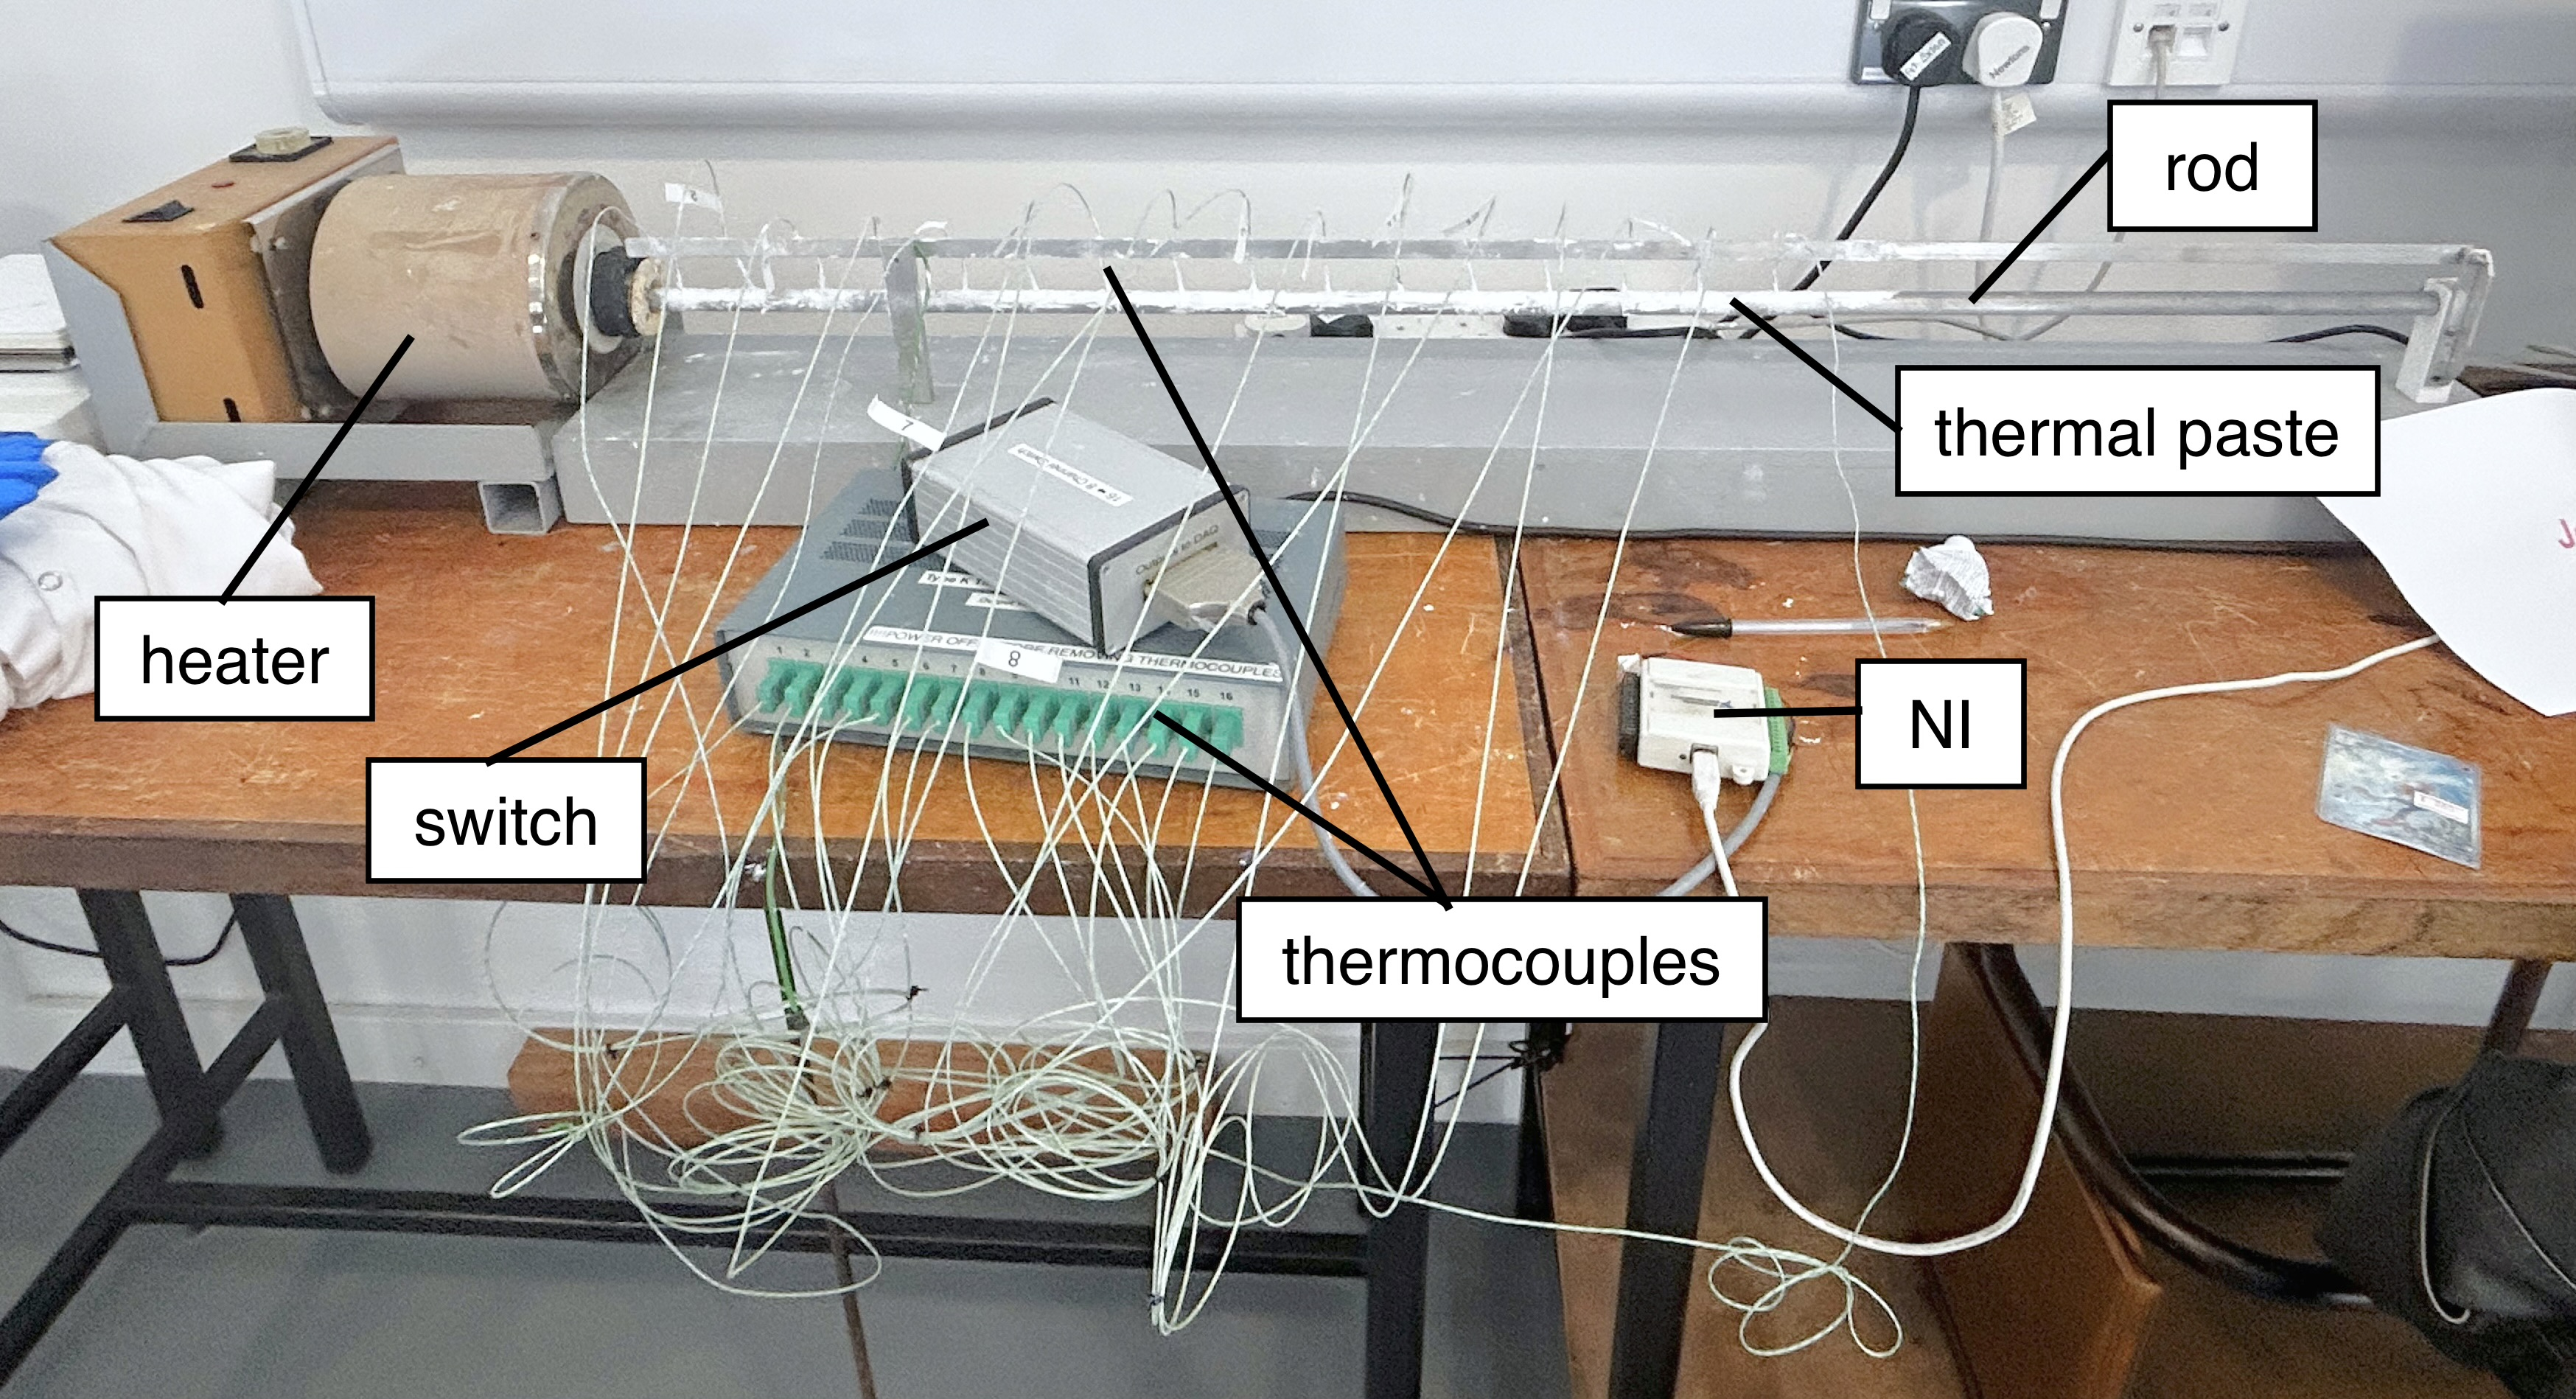
\includegraphics[width=.95\linewidth]{CoolNewton_setup.JPG}
  \caption{Experimental setup with equipment labels.}
  \label{fig:1}
\end{figure}

One end of an aluminium rod was inserted into a furnace, while the opposite end extended far enough to remain at ambient (room) temperature, acting as the external bath. Sixteen thermocouples were placed along the rod at a uniform spacing of 5 cm, beginning at the furnace end. Thermal paste was applied both to the thermocouple notches and to the exposed wire ends to improve thermal contact and ensure accurate readings. The thermocouples were connected to an 8-way switching box, which was in turn connected to a National Instruments USB-6008 data acquisition device.

\subsection{NI Setup}

Since the USB-6008 provides only eight analogue input channels while the experiment required sixteen thermocouple readings, the switching box was used to measure and stack two sets of eight channels onto a single set of inputs. Acquisition code was written to accommodate this. The channels were configured as single-ended (rather than the default differential mode) \cite{ucd2026niusb6008}:

\begin{lstlisting}
myADC = ADC()
myDAC = DAC(0)

myADC.addChannels([0,1,2,3,4,5,6,7], ADC_mode='DAQmx_Val_RSE')
\end{lstlisting}

Sixteen readings were then acquired by toggling the switching box between its two states, with 0 V selecting thermocouples 1-8, and 5 V selecting thermocouples 9-16.

\begin{lstlisting}
def thermocouple_16loop():
    voltages=np.zeros(16)

    myDAC.writeVoltage(0)
    time.sleep(0.05)
    set1=myADC.sampleVoltages(1)
    for i in range(8):
        voltages[i]=set1[i][0]

    myDAC.writeVoltage(5)
    time.sleep(0.05)
    set2=myADC.sampleVoltages(1)
    for i in range(8):
        voltages[i+8]=set2[i][0]

    myDAC.writeVoltage(0)
    return voltages
\end{lstlisting}

The function first creates an empty 16-element array, then records the first eight thermocouple voltages with the switch at 0 V, allowing 0.05 s for the switch to settle before each read, before repeating the process for the remaining eight thermocouples with the switch at 5 V. The switch is returned to 0 V at the end of each run in preparation for the next set of measurements.

\subsection{Calibration \& Data Acquisition}

To convert the raw NI voltage readings into temperatures, each thermocouple was calibrated individually. The sixteen thermocouples were bundled together and immersed in a beaker of water heated by kettle. The water's temperature was measured directly with a thermometer, while the corresponding thermocouple voltages were recorded using the acquisition loop defined. Paired thermometer-voltage readings were then taken continuously as the water cooled to room temperature. A linear fit of temperature against voltage, $T=V\cdot m + c$,was performed for each thermocouple individually, and the resulting slope $m$ and intercept $c$ were used to convert all subsequent voltage measurements from that thermocouple into temperature.

Two runs were then recorded. In the uniform run, the rod began at room temperature before the furnace was switched on. In the non-uniform run, the centre of the rod was first heated locally with a hairdryer before the furnace was switched on. Both runs lasted 75 minutes, with all sixteen thermocouples read and logged once every 60 seconds.

\subsection{Data Analysis}

Three measurements were calculated from the calibrated temperature data: the effective oven temperature, the steady-state temperature profile, and the rates of entropy transfer and production.

\subsubsection{Effective Oven Temperature}

The furnace's dial markings do not reliably indicate the true boundary temperature seen by the rod, since it does not account for ambient losses, contact resistance, or insulation effects. The true value $T_L$ was instead obtained from the measured steady-state profile using \Cref{eq:4}, rearranged by taking the natural logarithm of both sides:

\vspace{-3ex}
\begin{equation} \label{eq:8}
  \ln[T(z)-T_R] = \ln(T_L-T_R) - \beta z
\end{equation}

A plot of $\ln[T(z)-T_R]$ against the thermocouple positions $z$ is therefore linear, with a slope of $-\beta$ and intercept $\ln(T_L-T_R)$. $T_L$ was determined by extrapolating this linear fit to $z=0$, rather than reading directly from any single thermocouple as none was located exactly at the furnace boundary.

\subsubsection{Steady-State Temperature Profile}

The full time evolution of the temperature distribution was visualized with a 3D waterfall plot, with axes of time $t$, position $z$, and temperature $T$, each curve corresponding to one thermocouple. This used the calibrated temperature data directly, requiring no further calculation.

\subsubsection{Entropy Transfer and Production} \label{sec:2.3.3}

The rates of entropy transfer across the rod's boundary ($d_eS/dt$) and entropy production within it ($d_iS/dt$), were evaluated using expressions written in terms of experimentally accessible quantities:

\vspace{-3ex}
\begin{equation} \label{eq:9}
\begin{split}
\frac{d_eS}{dt} \propto\ 
&\int_0^L \frac{1}{T}\frac{\partial^2 T}{\partial z^2}\,dz 
- \int_0^L \frac{1}{T^2}\left(\frac{\partial T}{\partial z}\right)^2 dz \\
&- \frac{2H}{\lambda r}\int_0^L \frac{1}{T}(T-T_R)\,dz
\end{split}
\end{equation}

\begin{equation} \label{eq:10}
  \frac{d_i S}{dt} \propto \int^L_0 \frac{1}{T^2} \left( \frac{\partial T}{\partial z} \right)^2 dz
\end{equation}

To avoid the numerical instability of computing a second spatial derivative due to the low density of experimental data, a discrete version of \Cref{eq:9,eq:10} was used utilising experimental values: the measured thermocouple temperatures $T_i$, thermocouple spacing $l$, and the fitted decay constant $\beta$:

\vspace{-3ex}
\begin{equation}\label{eq:11}
\begin{split}
\frac{d_eS}{dt} \propto\ 
&-\frac{1}{l}\frac{1}{T_0}(T_1-T_0) + \frac{1}{l}\frac{1}{T_n}(T_n-T_{n-1}) \\
&- \beta^2 l\sum_{i=1}^{n-1}\left(1-\frac{T_n}{T_i}\right)
\end{split}
\end{equation}
\vspace{-1ex}
\begin{equation} \label{eq:12}
  \frac{d_i S}{dt} \propto -\frac{1}{l} \sum^{n-1}_{i=0} (T_{i+1} - t_i) \left( \frac{1}{T_{i+1}} - \frac{1}{T_i} \right)
\end{equation}

Here, $T_0 = T_L$ and $T_n = T_R$ denote the two fixed boundary temperatures, and all temperatures were expressed in Kelvin, since the $1/T$ terms require an absolute temperature scale. Results are presented as $d_iS/dt$ and $-d_eS/dt$, following the convention that makes both quantities converge to the same value and hence directly comparable to the steady-state with an established entropy minimum.

In practice, TCouple 16 had not fully relaxed to $T_R$ by the end of the either run, remaining several degrees above the room temperature the thermocouples were calibrated to. Since \Cref{eq:11,eq:12} assume the last measurement already sits at ambient boundary temperature, applying the measured $T_R$ readings would create a very large residiual gap between $d_iS/dt$ and $d_eS/dt$. To correct for this, "virtual thermocouples" were extended beyond TCouple 16 following the same exponential profile of \Cref{eq:4}, with the same spacing $z$, until the modelled temperature fell within a small tolerance of $T_R$.

\section{Results} \label{sec:3}

\subsection{Calibration} \label{sec:3.1}

The calibration data for all sixteen thermocouples taken for seven reference temperatures, from room temperature (20.2 °C) to kettle-boiled temperature (76.5 °C), are shown in \Cref{fig:2} alongside their individual fits. All sixteen curve fits are visually linear over the full measured voltage range.

\begin{figure}[H]
  \centering
  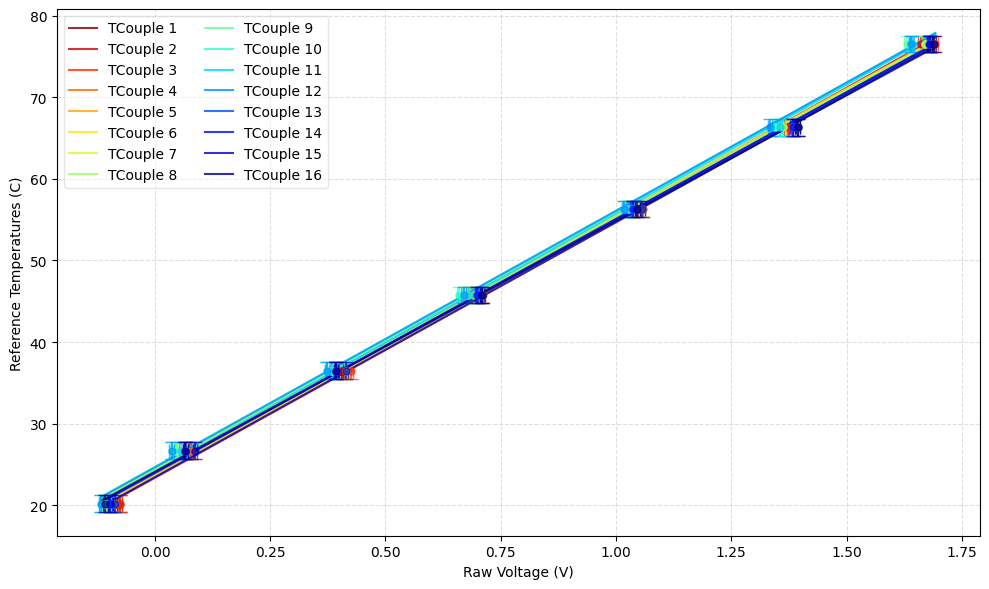
\includegraphics[width=.95\linewidth]{NCool_calibplot.png}
  \caption{Calibration plot.}
  \label{fig:2}
\end{figure}

Each thermocouple was individually fitted to $T=V \cdot m + c$ by least squares regression, using the manufacturer-specified thermometer 1 °C uncertainty. The resulting uncertainty on each fitted slope $\sigma_m$ and intercept $\sigma_c$, together with their covariance Cov($m,c$), were then propagated onto the uncertainty on the measured temperatures with:

\vspace{-3ex}
\begin{equation} \label{eq:13}
  \sigma_T^2 = V^2 \sigma_m^2 + \sigma_c^2 + 2V \text{Cov}(m,c)
\end{equation}

\subsection{Effective Oven Temperature} \label{sec:3.2}

\Cref{fig:3} shows $\ln[T(z)-T_R]$ plotted against the thermocouple positions ($z$) for both the uniform and non-uniform runs. Both sets of data were fitted with a straight line over the full 0.05-0.80 m range, consistent with the exponential steady-state profile described in \Cref{eq:4}. 

\begin{figure}[H]
  \centering
  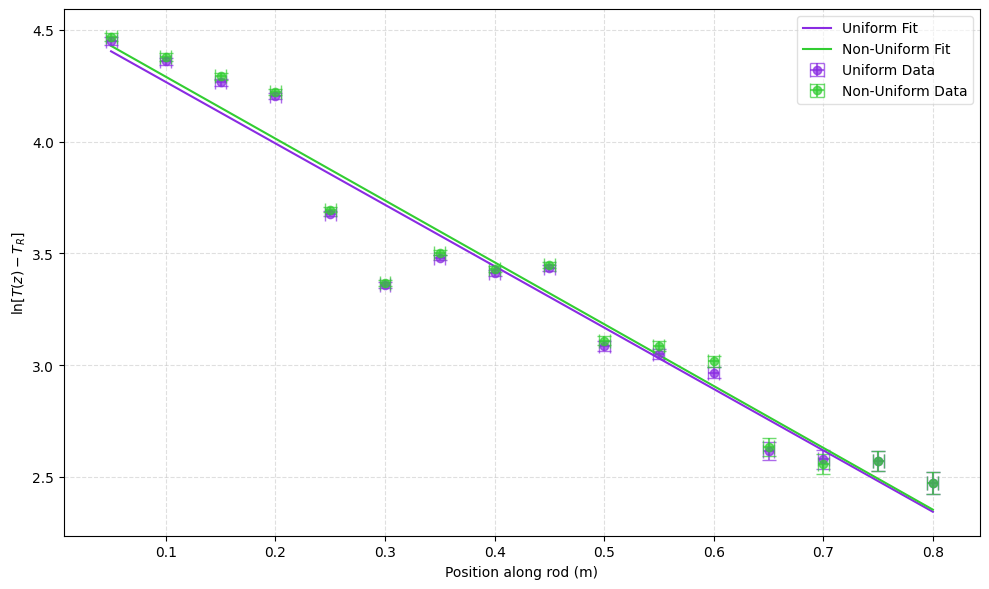
\includegraphics[width=.95\linewidth]{NCool_oventemp.png}
  \caption{Effective oven temperature plot.}
  \label{fig:3}
\end{figure}

Extrapolating each linear fit to z=0 gives the values of:

\vspace{-5ex}
\begin{gather*}
  \beta_{\text{unif}} = 2.7458\; m^{-1} \qquad \beta_{\text{non-unif}} = 2.7656\; m^{-1}\\
  T_{L,\text{unif}} = 113.99\; ^{\circ}C \qquad T_{L,\text{non-unif}}= 116.39\; ^{\circ}C
  \vspace{-1ex}
\end{gather*}

The uncertainties on $\beta$ and $T_L$ were determined using the corresponding weighted fit of \Cref{eq:8}. Per-point weighted uncertainties were given by extending the propagation of the calibration uncertainty from \Cref{eq:13}, giving $\sigma_{\ln[T(z)-T_R]}=\sigma_T / (T-T_R)$, and thus the corrected values with uncertainties:

\vspace{-4ex}
\begin{gather*}
  \beta_{\text{unif}} = 2.8216\;\pm 0.0264\; m^{-1} \\
  T_{L,\text{unif}} = 113.99\;\pm 0.88\; ^{\circ}C \\
  \beta_{\text{non-unif}} = 2.8042\;\pm 0.0261\; m^{-1} \\
  T_{L,\text{non-unif}} = 115.21\;\pm 0.90\; ^{\circ}C
\end{gather*}

\subsection{Steady-State Temperature Profile} \label{sec:3.3}

The full time evolution of the distribution for both the uniform and non-uniform runs is shown in \Cref{fig:4}. In the uniform run, all sixteen thermocouples relax monotonically from room temperature toward their steady-state temperature values. In the non-uniform run, the midpoints that had been locally pre-heated show a temperature peak within the first $\sim-30$ minutes before decaying toward the same general profile shape as the uniform run and eventually relaxing again to their steady-state temperature values.

Both plots appear visually stationary for $t\gtrsim45$ mins. At the end of the recorded run ($t=74$ mins) the thermocouple nearest the furnace (TCouple 1) reads 105.76 °C for the uniform run and 125.13 °C for the non-uniform run.

\begin{figure}[!ht]
  \centering
  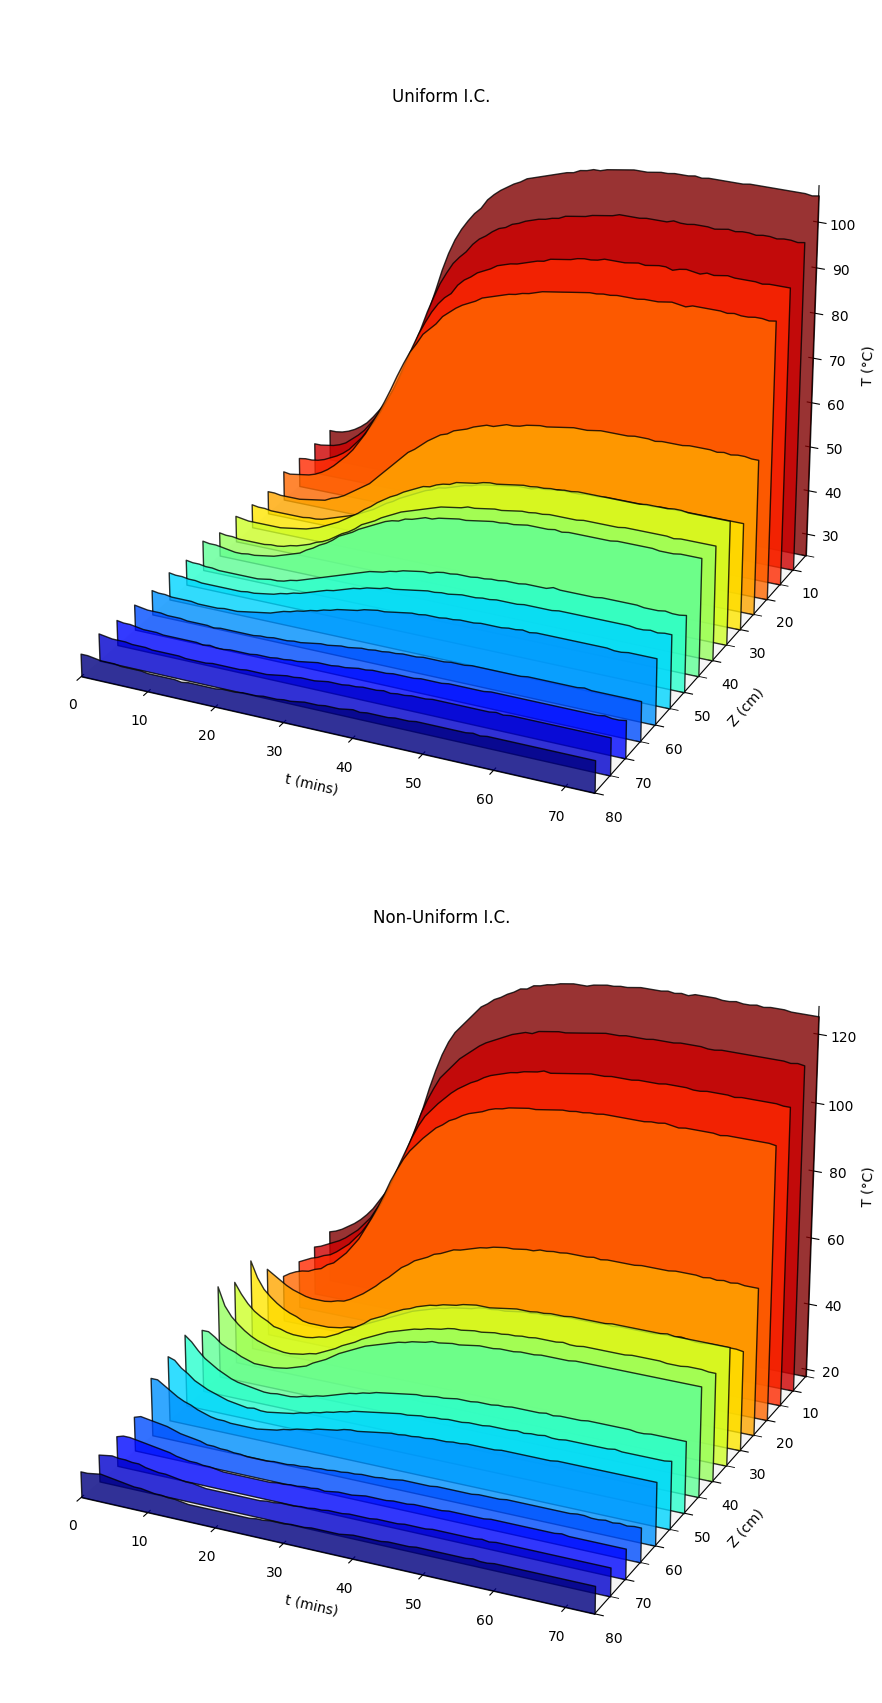
\includegraphics[width=\linewidth]{NCool_steadystate1.png}
  \caption{Steady-state plot for uniform (above) and non-uniform initial conditions (below).}
  \label{fig:4}
\end{figure}

\subsection{Entropy Transfer and Production} \label{sec:3.4}

\Cref{fig:5} shows $d_iS/dt$ and $-d_eS/dt$ as a function of time for both the uniform and non-uniform runs, computed from \Cref{eq:11,eq:12}. In both cases the condition of $d_iS/dt \ge 0$ as per the second law of thermodynamics was satisfied at every point. $d_iS/dt$ decreased monotonically from its initial value to a non-zero minimum corresponding to the steady state:

\vspace{-3ex}
\begin{align*}
  \left. \frac{d_iS}{dt}\right|_{unif}&:1.1395 \to 0.2047\\ 
  \left. \frac{d_iS}{dt}\right|_{non-unif}&:1.0227 \to 0.2148
\end{align*}

\vspace{2ex}
\begin{figure}[H]
  \centering
  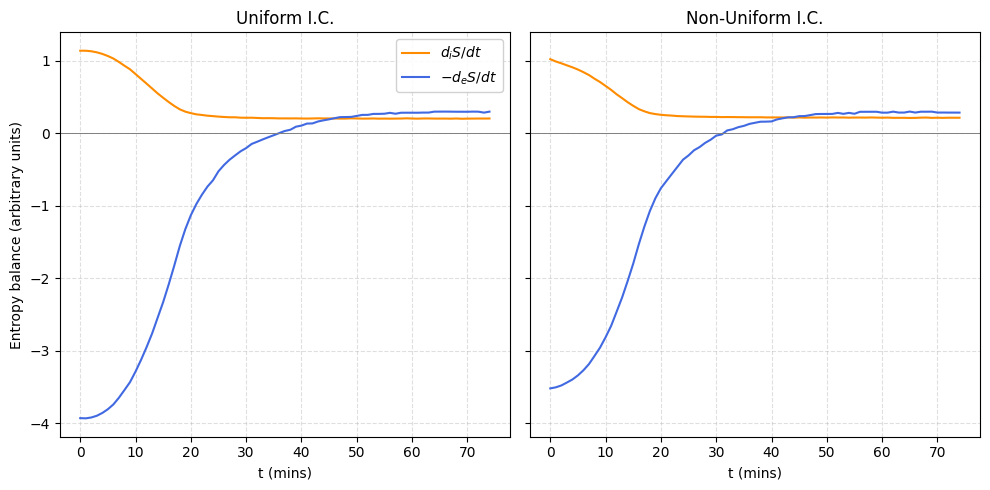
\includegraphics[width=\linewidth]{NCool_entropy.png}
  \caption{Entropy production and transfer rates for uniform and non-uniform initial conditions.}
  \label{fig:5}
\end{figure}

$-d_eS/dt$ begins negative in both runs and increases over time, approaching the corresponding $d_iS/dt$ curve as $t$ increases and settling slightly above it by the end of the run at steady-state:

\vspace{-3ex}
\begin{align*}
  \left. \frac{-d_eS}{dt}\right|_{unif}&:-3.9282 \to 0.2992\\ 
  \left. \frac{-d_eS}{dt}\right|_{non-unif}&:-3.8876 \to 1.1890
\end{align*}

Since $d_iS/dt$ and $d_eS/dt$ are nonlinear functions for a large range of temperatures for many individual thermocouples, their uncertainty was obtained with Monte Carlo propagation rather than analytic. Every input alongside their uncertainties ($T_i(t)$, $T_L$, $T_room$, and $\beta$) were resampled 500 times from a Gaussian distribution centered on its measured or fitted values. The resulting mean and standard deviation of the resulting entropy rates gave:

\vspace{-3ex}
\begin{align*}
  \left. \frac{d_iS}{dt}\right|_{u}&:1.142\;\pm 0.032 \to 0.2086\;\pm 0.0091\\ 
  \left. \frac{d_iS}{dt}\right|_{non-u}&:1.025\;\pm 0.027 \to 0.2186\;\pm 0.009\\[2ex]
  \left. \frac{-d_eS}{dt}\right|_{u}&:-3.919\;\pm 0.056 \to 0.3329\;\pm 0.093\\ 
  \left. \frac{-d_eS}{dt}\right|_{non-u}&:-3.504\;\pm 0.052 \to 0.3114\;\pm 0.094
\end{align*}

\section{Analysis and Discussion} \label{sec:4}

The fitted decay constant $\beta$ showed the strongest agreement with theory discussed in \Cref{sec:1.1}. Because it depends solely on the material and geometric properties of the rod and its surroundings ($\beta=\sqrt{2H/\lambda r}$), it is expected to be mostly independent of the initial conditions. This independence was observed in \Cref{sec:3.2}: the values obtained from the fitted slopes $\beta_{\text{unif}} = 2.8216\;\pm 0.0264\; m^{-1}$ and $\beta_{\text{non-unif}} = 2.8042\;\pm 0.0261\; m^{-1}$, agree within their combined uncertainties ($\Delta \beta = 0.0174\;m^{-1}$ vs. $\sigma_{\Delta\beta}=0.0371\;m^{-1}$). This confirmed that despite differing initial heating conditions, both experimental runs convereged to nearly identical values of a parameter only dependent on the apparatus itself.

The heater temperature $T_L$ also showed agreement: $113.99\;\pm 0.88\; ^{\circ}C$ (uniform) and $115.21\;\pm 0.90\; ^{\circ}C$ (non-uniform) and a difference in calculated $T_L$ of $\Delta T_L = 1.22\;^{\circ}C$ within a combined uncertainty of $\sigma_{\Delta T_L}=1.259\;^{\circ}C$. The main divergence happened in readings from the thermocouple closest to the heater (TCouple 1), which read 105.76 °C (uniform) and 125.13 °C (non-uniform) with a difference of 19.37 °C.

Since $\beta$ remained mostly unaffected despite the large temperature shift, it is unlikely that the discrepancy came from the rod material or geometric behaviours. Instead it is more likely that they are due to local differences in the heater-rod junction between both runs, such as residual heat in the furnace or incomplete cooling of the rod before the non-uniform run due to lab time constraints. However, this discrepancy shows the advantage of extrapolating $T_L$ from the full linear fit as it considers the entire profile rather than reading from a single near-furnace sensor.

The entropy results from \Cref{sec:3.4} directly verified the theory discussed in \Cref{sec:1.2,sec:1.3}. The condition $d_iS/dt \ge 0$ was satisfied across all measurement points, confirming the second law of thermodynamics (\Cref{eq:7}).For both initial conditions, $d_iS/dt$ decreased monotonically from its initial value toward a non-zero steady-state minimum, supporting Prigogine's principle (\Cref{sec:1.3}). Specifically, $d_iS/dt$ settled at $0.2086\;\pm 0.0091$ (uniform) and $0.2186\;\pm 0.009$ (non-uniform), both bounded away from zero. These results agree within their combined uncertainty ($\sigma_{\Delta d_iS}=0.0128$), demonstrating that the steady-state is determined by boundary conditions rather than initial states.

Discreprancies arise when analysing $-d_eS/dt$. The theoretical steady-state requires $-d_eS/dt \to d_iS/dt$ exactly, but in both runs $-d_eS/dt$ instead overshoots. It rises strongly from the negative values and settles slightly above $d_iS/dt$: $0.3329\;\pm 0.093$ versus $d_iS/dt = 2086\;\pm 0.0091$ (uniform), and $0.3114\;\pm 0.094$ versus $d_iS/dt = 0.2186\;\pm 0.009$ (non-uniform). For the uniform run, this excess is outside the Monte Carlo uncertainty, and for the non-uniform run the curves almost overlap. 

Further sources of error unquantified in $\beta$, $T_L$, and entropy rates likely contributed to residual discrepancies. Slight thermocouple movement in between the readings and frayed sensor may have not allowed them to seat at the same depth, introducing small spatial uncertainties not captured in $\beta$ nor $T_L$. Uneven application of thermal paste may have also introduced minor local thermal resistances or unbalanced readings uncorrected by the beaker-water calibration. Finally, as noted beforehand, unequal initial thermal states of the rod and furnace introduced a systematic offset between datasets, which could only be partially fixed by extrapolating the effective furnace temperature.

These error show clear possibilities for possible improvements in future iterations of this experiment. Allowing the heater and rod to return completely to room temperature between runs would eliminate the initial value thermal discrepancies. Extending run durations beyond 75 minutes would ensure the system reaches true steady-state. Although constrained by the setup in the UCD laboratory, the addition of thermocouples particularly near the furnace where the temperature gradient is steepest (\Cref{fig:4}), would significantly improve samples. Finally, conducting multiple trials across different heater temperatures would improve the reliability and better validate the theory behind it.

\section{Conclusion}

This experiment used an aluminium rod subjected to a fixed furnace temperature and lateral Newtonian heat losses to investigate the approach to nonequilibrium steady-state, and to test Prirogine's minimum entropy production theorem that describes the balance in entropy production and transfer. Two runs with uniform and non-uniform initial heating conditions were conducted, analysed, and compared.

The steady-state temperature profile was well described by the expected exponential form in either run, and the extracted decay constant $\beta$, which is dependent on experimental geomtery only, agreed between the runs within the uncertainty ($2.8216\;\pm 0.0264\; m^{-1}$ and $2.8042\;\pm 0.0261\; m^{-1}$). This is despite a large difference in direct readings of temperature near the furnace between runs, most likely due to insufficient cooling between sessions rather than any change in the apparatus itself. The entropy production rate $d_iS/dt$ was determined to satisfy the second law of thermodynamics at all times in both runs and decreased monotonically towards a non-zero minimum corresponding with the steady-state ($0.2086\;\pm 0.0091$ and $0.2186\;\pm 0.009$). The entropy transfer term $-d_eS/dt$ rose from strong negative values, crossed $d_iS/dt$, and settled slightly above it by the end of the runs instead of converging onto it exactly, and was shown to be significantly more sensitive to the fittedvalue of $\beta$ than $d_iS/dt$, indicating that the rod might not have yet reached a true steady-state within the 75 minute measurement window, particularly near the ambient far end despite the temperature profile graph suggesting otherwise.

Overall, the results support the theoretical discussion: the steady-state profile and the entropy production and dominated by the fixed boundary conditions of the system rather than its initial state, and the second law of thermodynamics and minimum entropy production theorem both hold within experimental uncertainties. The main limitations discussed identified concrete improvements for any repeats of this experiment.



%%%%%%%%%%%%%%%%%%%%

% References - switch to single column
\onecolumn

\bibliographystyle{IEEEtran}
\bibliography{PHYC40600ref} \label{sec:ref}

\newpage

% Appendix - single column
\section*{Appendix} \label{sec:A}
\addcontentsline{toc}{section}{Appendix}

\subsection*{Tables}
\addcontentsline{toc}{subsection}{Tables}

\begin{table}[H]
\centering
\caption{Slopes and intercepts and respective uncertainties for the calibration plot for \Cref{sec:3.1}.}
\label{tab:1}
\begin{tabular}{|
>{\columncolor[HTML]{EFEFEF}}c |c|c|c|c|}
\hline
TCouple & \cellcolor[HTML]{EFEFEF}slope m (C/V) & \cellcolor[HTML]{EFEFEF}$\sigma_m$ slope (C/V) & \cellcolor[HTML]{EFEFEF}intercept c (C) & \cellcolor[HTML]{EFEFEF}$\sigma_c$ intercept (C) \\ \hline
1       & 31.4201                               & 0.6199                                         & 23.5024                                 & 0.5966                                           \\ \hline
2       & 31.6219                               & 0.6238                                         & 23.724                                  & 0.5932                                           \\ \hline
3       & 31.3196                               & 0.6179                                         & 23.3561                                 & 0.5988                                           \\ \hline
4       & 31.3226                               & 0.6179                                         & 23.5892                                 & 0.5953                                           \\ \hline
5       & 30.8565                               & 0.6089                                         & 24.4498                                 & 0.5823                                           \\ \hline
6       & 31.051                                & 0.6126                                         & 24.4679                                 & 0.582                                            \\ \hline
7       & 31.0862                               & 0.6133                                         & 23.6522                                 & 0.5944                                           \\ \hline
8       & 31.0574                               & 0.6127                                         & 24.3245                                 & 0.5841                                           \\ \hline
9       & 31.6508                               & 0.6245                                         & 24.3006                                 & 0.5845                                           \\ \hline
10      & 31.351                                & 0.6185                                         & 24.7002                                 & 0.5785                                           \\ \hline
11      & 31.6125                               & 0.6237                                         & 24.1059                                 & 0.5875                                           \\ \hline
12      & 31.4322                               & 0.6201                                         & 24.6543                                 & 0.5792                                           \\ \hline
13      & 31.0608                               & 0.6128                                         & 23.9839                                 & 0.5893                                           \\ \hline
14      & 31.0607                               & 0.6128                                         & 24.0076                                 & 0.5889                                           \\ \hline
15      & 31.2542                               & 0.6165                                         & 23.4353                                 & 0.5976                                           \\ \hline
16      & 30.7427                               & 0.6064                                         & 24.1047                                 & 0.5874                                           \\ \hline
\end{tabular}
\end{table}

\begin{table}[H]
\centering
\caption{Clean summary table for the $\beta$, $T_L$, and entropy values.}
\label{tab:2}
\begin{tabular}{|
>{\columncolor[HTML]{EFEFEF}}c |c|c|}
\hline
Quantity                 & \cellcolor[HTML]{EFEFEF}\textbf{Uniform} & \cellcolor[HTML]{EFEFEF}\textbf{Non-uniform} \\ \hline
$\beta$ ($m^{-1}$)       & 2.8216 ± 0.0264                          & 2.8042 ± 0.0261                              \\ \hline
$T_L$ (°C)               & 113.99 ± 0.88                            & 115.21 ± 0.90                                \\ \hline
$d_iS/dt$, t=0           & 1.142 ± 0.03161                          & 1.025 ± 0.02708                              \\ \hline
$d_iS/dt$, steady state  & 0.2086 ± 0.009139                        & 0.2186 ± 0.009331                            \\ \hline
$-d_eS/dt$, t=0          & -3.919 ± 0.05582                         & -3.504 ± 0.05173                             \\ \hline
$-d_eS/dt$, steady state & 0.3329 ± 0.09272                         & 0.3114 ± 0.09395                             \\ \hline
\end{tabular}
\end{table}

\addcontentsline{toc}{subsection}{Code}

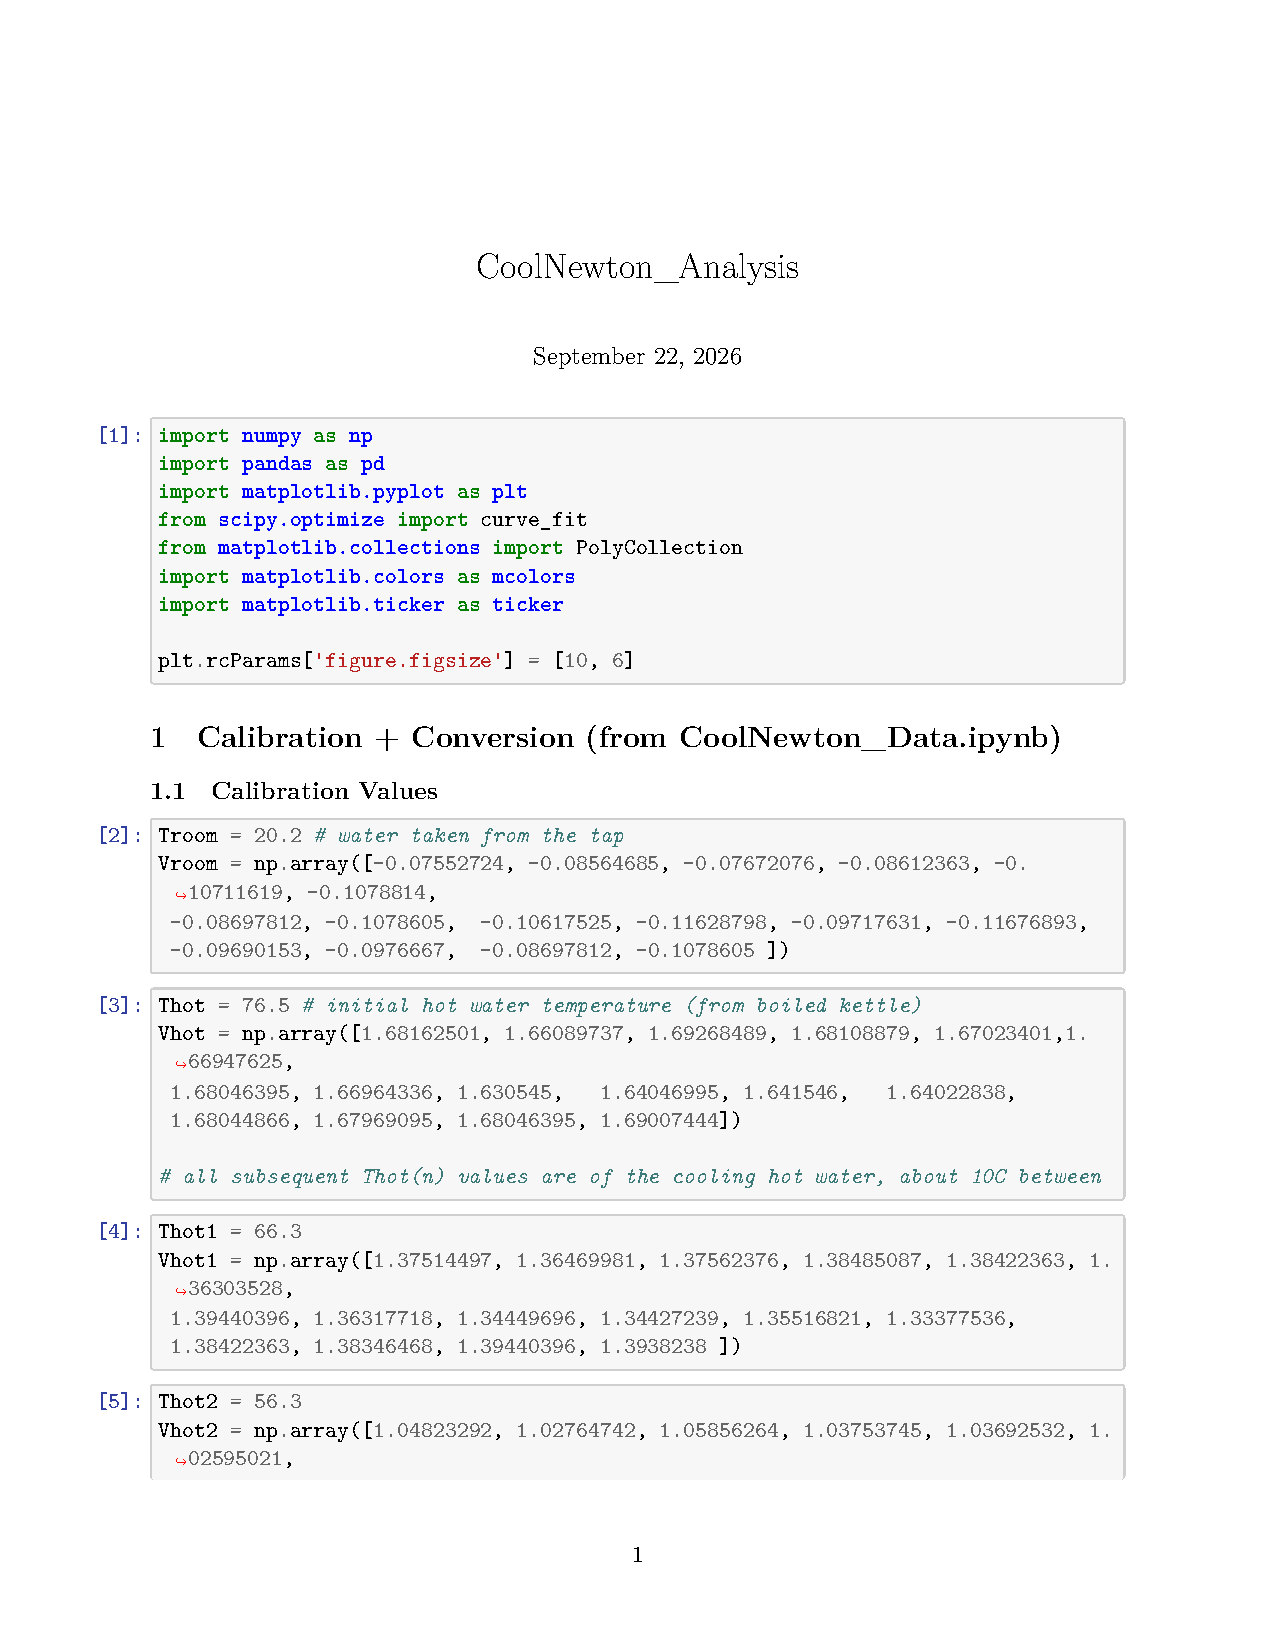
\includepdf[pages={1-3,6-7,10-13,16-19}]{CoolNewton_Analysis.pdf}

\end{document}